
\chapter{找规律}
\label{chap:pattern}

\section{序列}
\label{sec:series-pattern}

\begin{example}[等差数列]
  \begin{align*}
    3,\quad 5,\quad 7,\quad 9,\quad 11,\quad ?
  \end{align*}
\end{example}

\begin{example}[等比数列]
  \begin{align*}
    3,\quad 6,\quad 12,\quad 24,\quad 48,\quad 96,\quad ?
  \end{align*}
\end{example}

\begin{example}[双数列]
  \begin{align*}
    1,\quad 2,\quad 3,\quad 4,\quad 5,\quad 8,\quad 7,\quad ?
  \end{align*}
\end{example}
\begin{proof}[提示]\mbox{}\par
  \begin{center}
    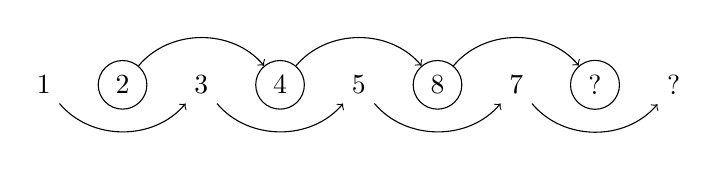
\begin{tikzpicture}[scale=1.0]
      \node(N1) at (1,0) {1};
      \node[draw,circle](N2) at (2,0) {2};
      \node(N3) at (3,0) {3};
      \node[draw,circle](N4) at (4,0) {4};
      \node(N5) at (5,0) {5};
      \node[draw,circle](N8) at (6,0) {8};
      \node(N7) at (7,0) {7};
      \node[draw,circle](N16) at (8,0) {?};
      \node(N9) at (9,0) {?};
      \foreach \x/\y in{N1/N3,N3/N5,N5/N7,N7/N9}{
        \draw[->](\x)edge[bend right=50](\y);
      }
      \foreach \x/\y in{N2/N4,N4/N8,N8/N16}{
        \draw[->](\x)edge[bend left=50](\y);
      }
    \end{tikzpicture}
  \end{center}
  分割成两个数列。
\end{proof}

\begin{example}[双数列]
  \begin{align*}
    8,\quad 14,\quad 10,\quad 12,\quad 12,\quad 9,\quad 14,\quad 5,\quad ?
  \end{align*}
\end{example}
\begin{proof}[提示]\mbox{}\par
  \begin{center}
    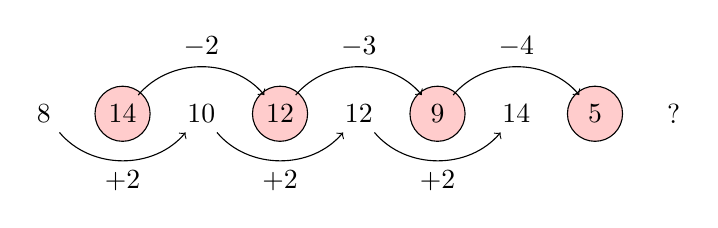
\begin{tikzpicture}[scale=1.0]
      \foreach \x in {2,4,6,8}{
        \draw[fill=red!20](\x,0)circle(.35);
      }
      \foreach \x/\t in{1/8, 2/14, 3/10, 4/12, 5/12, 6/9, 7/14, 8/5, 9/?}{
        \node(N\x) at(\x,0) {\t};
      }
      \foreach \x/\y/\t in{1/3/2, 3/5/2, 5/7/2}{
        \draw[->](N\x)edge[bend right=50]node[below]{$+\t$}(N\y);
      }
      \foreach \x/\y/\t in{2/4/2, 4/6/3, 6/8/4}{
        \draw[->](N\x)edge[bend left=50]node[above]{$-\t$}(N\y);
      }
    \end{tikzpicture}
  \end{center}
  分割成两数列。
\end{proof}

\begin{example}[三数列]
  \begin{align*}
    1,\quad 2,\quad 3,\quad 4,\quad 4,\quad 4,\quad 7,\quad 8,\quad 6,\quad 10,\quad 16,\quad 9,\quad ?
  \end{align*}
\end{example}
\begin{proof}[提示]\mbox{}\par
  \begin{center}
    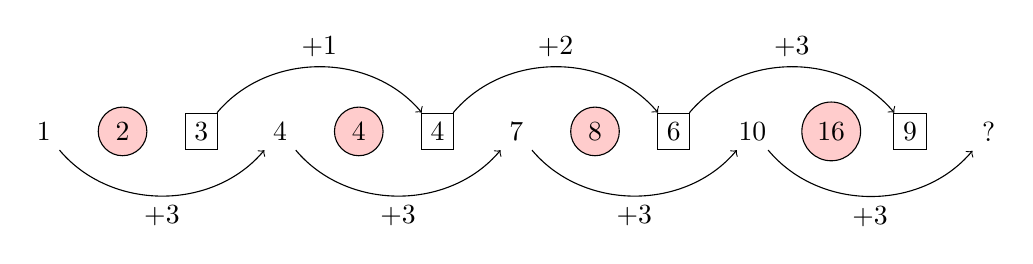
\begin{tikzpicture}[scale=1.0]
      \node(N1) at(1, 0){1};
      \node[draw,circle,fill=red!20](N2) at(2, 0){2};
      \node[draw](N3) at(3, 0){3};
      \node(N4) at(4, 0){4};
      \node[draw,circle,fill=red!20](N5) at(5, 0){4};
      \node[draw](N6) at(6, 0){4};
      \node(N7) at(7, 0){7};
      \node[draw,circle,fill=red!20](N8) at(8, 0){8};
      \node[draw](N9) at(9, 0){6};
      \node(N10)at(10,0){10};
      \node[draw,circle,fill=red!20](N11)at(11,0){16};
      \node[draw](N12)at(12,0){9};
      \node(N13)at(13,0){?};
      \foreach \x/\y in {N1/N4, N4/N7, N7/N10,N10/N13}{
        \draw[->](\x)edge[bend right=50]node[below]{$+3$}(\y);
      }
      \foreach \x/\y/\t in {N3/N6/$+1$, N6/N9/$+2$, N9/N12/$+3$}{
        \draw[->](\x)edge[bend left=50]node[above]{\t}(\y);
      }
    \end{tikzpicture}
  \end{center}
  分割成三个数列。
\end{proof}

\begin{example}[双循环]
  \begin{align*}
    1,\quad 2,\quad 4,\quad 5,\quad 10,\quad 11,\quad 22,\quad 23,\quad 46,\quad ?
  \end{align*}
\end{example}
\begin{proof}[提示]\mbox{}\par
  \begin{center}
    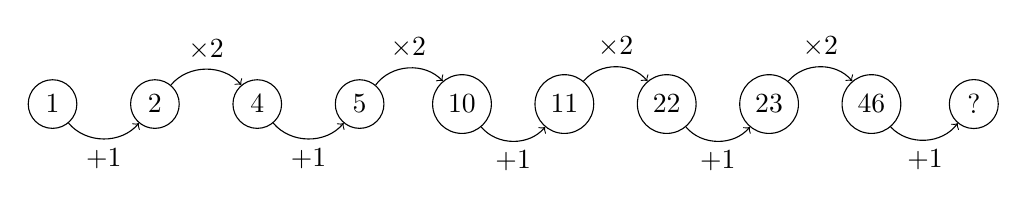
\begin{tikzpicture}[scale=1.0]
      \foreach \x/\y in {1/1, 2/2, 3/4, 4/5, 5/10, 6/11, 7/22, 8/23, 9/46, 10/?}{
        \node[draw,circle](N\x) at(1.3*\x,0) {\y};
      }
      \foreach \x/\y in {N1/N2,N3/N4,N5/N6,N7/N8,N9/N10}{
        \draw[->](\x)edge[bend right=50]node[below]{$+1$}(\y);
      }
      \foreach \x/\y in {N2/N3,N4/N5,N6/N7,N8/N9}{
        \draw[->](\x)edge[bend left=50]node[above]{$\times2$}(\y);
      }
    \end{tikzpicture}
  \end{center}
  以$+1,\ \times2$的模式循环。
\end{proof}

\begin{example}[两级规律]
  \begin{align*}
    1,\quad 3,\quad 7,\quad 15,\quad 31,\quad 63,\quad 127,\quad ?
  \end{align*}
\end{example}
\begin{proof}[提示]通过两级等差等比关系可得。
  \begin{center}
    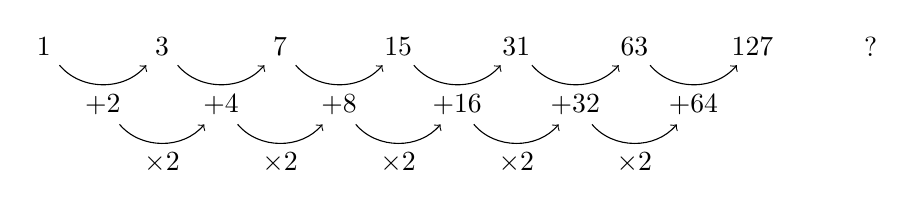
\begin{tikzpicture}[scale=1.0]
      \foreach \x/\y in{1/1, 2/3, 3/7, 4/15, 5/31, 6/63, 7/127, 8/?}{
        \node(N\x) at (1.5*\x, 0) {\y};
      }
      \foreach \x/\y/\t in{1/2/2, 2/3/4, 3/4/8, 4/5/16, 5/6/32, 6/7/64}{
        \draw[->](N\x)edge[bend right=50]node(NN\x)[below]{$+\t$}(N\y);
      }
      \foreach \x/\y in{1/2, 2/3, 3/4,4/5,5/6}{
        \draw[->](NN\x)edge[bend right=50]node[below]{$\times2$}(NN\y);
      }
    \end{tikzpicture}
  \end{center}
  \note 实际上,若熟悉2的各次幂,也容易得到其规律:
  \begin{align*}
    2^0&=1, & 2^1&=2,  & 2^2&=4\\
    2^3&=8, & 2^4&=16, & 2^5&=32\\
    2^6&=64,& 2^7&=128,& 2^8&=256
  \end{align*}
  所以第$n$项的公式为$2^n-1$。
\end{proof}

\begin{example}[三级规律]
  \begin{align*}
    1,\quad 2,\quad 3,\quad 5,\quad 11,\quad 35,\quad ?
  \end{align*}
\end{example}
\begin{proof}[提示]分三层分析。
  \begin{center}
    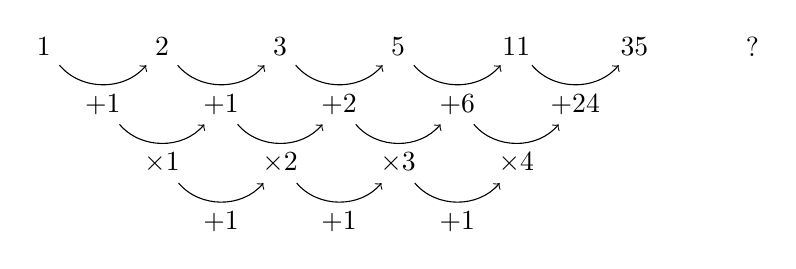
\begin{tikzpicture}[scale=1.0]
      \foreach \x/\y in{1/1, 2/2, 3/3, 4/5, 5/11, 6/35, 7/?}{
        \node(N\x) at (1.5*\x, 0) {\y};
      }
      \foreach \x/\y/\t in{1/2/1, 2/3/1, 3/4/2, 4/5/6, 5/6/24}{
        \draw[->](N\x)edge[bend right=50]node(NN\x)[below]{$+\t$}(N\y);
      }
      \foreach \x/\y/\t in{1/2/1, 2/3/2, 3/4/3, 4/5/4}{
        \draw[->](NN\x)edge[bend right=50]node(NNN\x)[below]{$\times\t$}(NN\y);
      }
      \foreach \x/\y in{1/2,2/3,3/4}{
        \draw[->](NNN\x)edge[bend right=50]node[below]{$+1$}(NNN\y);
      }
    \end{tikzpicture}
  \end{center}
  按此规律,?处应为$35 + 24\times(4+1)=155$。
\end{proof}

\begin{example}[斐波那契数列,Fibonacci sequence]
  \begin{align*}
    1,\quad 1,\quad 2,\quad 3,\quad 5,\quad 8,\quad 13,\quad 21,\quad 34,\quad 55,\quad 89
  \end{align*}
  从第3项起,每项是其前两项的和。
  \begin{center}
    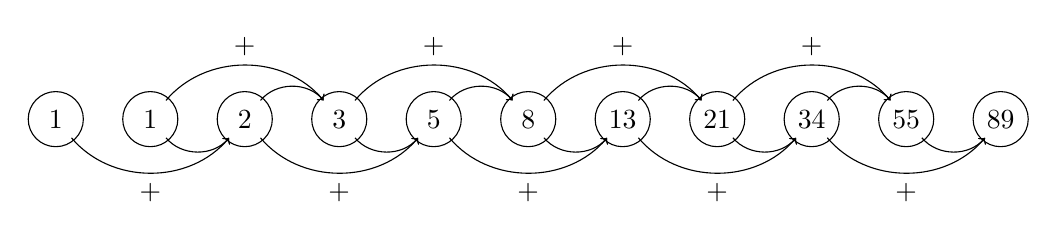
\begin{tikzpicture}[scale=1.0]
      \foreach \x/\t in{1/1, 2/1, 3/2, 4/3, 5/5, 6/8, 7/13, 8/21, 9/34, 10/55, 11/89}{
        \node(N\x) at(1.2*\x, 0) {\t};
        \draw(N\x)circle(.35);
      }
      \foreach \x/\y/\t in {1/3/+,2/3/, 3/5/+,4/5/, 5/7/+,6/7/, 7/9/+,8/9/, 9/11/+,10/11/}{
        \draw[->](N\x)edge[bend right=50]node[below]{$\t$}(N\y);
      }
      \foreach \x/\y/\t in {2/4/+,3/4/, 4/6/+,5/6/, 6/8/+,7/8/, 8/10/+,9/10/}{
        \draw[->](N\x)edge[bend left=50]node[above]{$\t$}(N\y);
      }
    \end{tikzpicture}
  \end{center}
\end{example}

\subsection{外观数列}
\label{sec:look-and-say-sequence}

\begin{example}[外观数列,Look-and-say Sequence,Morris Number Sequence]
  \begin{align*}
    1,\quad 11,\quad 21,\quad 1211,\quad 111221,\quad 312211,\quad 13112221,\quad ?
  \end{align*}
\end{example}
\begin{proof}[说明]
  该序列被称为外观数列,以$1$为开始,后一项是前一项的描述。如第二项$11$是关于第一项$1$的描述,即“$1$个$1$”;第三项$21$是关于第二项$11$的描述,即“$2$个$1$”;第四项$1211$是关于第三项$21$的描述,即“$1$个$2$,$1$个$1$”;第五项$111221$是关于第四项$1211$的描述,即“$1$个$1$,$1$个$2$,$2$个$1$”;以此类推。容易观察到,这个数列里只有数字$1,2,3$。Conway的cosmological theorem里证明了,这个数列邻近两项的比值收敛于一个常数:
  \begin{align*}
    \lim_{n\to\infty}\frac{L_{n+1}}{L_n}=\lambda
  \end{align*}
  此常数$\lambda$称为Conway常数,其值$\lambda\approx 1.303577269034$。

  以$22$开始的外观数列为:
  \begin{align*}
    22,\quad 22,\quad 22,\quad 22,\quad 22,\quad 22,\quad 22,\quad \cdots\cdots
  \end{align*}
  除此之外,以其它数开始的外观数列,都是不会循环的。
\end{proof}

\subsection{有形数}
\label{sec:figurate-number}

\begin{example}[三角形数,Triangular Number]三角形是指按如下方式组成正三角形的\tikz{\draw(0,0)circle(.1);}个数。
  \begin{center}\normalfont
    \begin{tikzpicture}[scale=1.0]
      \foreach \x/\y in{1/1,2/3,3/6,4/10,5/15,6/21,7/28}{
        \begin{scope}[shift={(.3*\y+ .3*\x,0)}]
          \node at(.15*\x+.15,-.5){$\y$};
          \setcounter{X}{0}
          \whiledo{\not{\value{X}>\x}}{%
            \setcounter{Y}{0}
            \whiledo{\value{Y}<\value{X}}{%
              \ifnum\numexpr\x=\theX
                \draw[fill=red!20](.3*\theX - .15*\theY,.3*\theY)circle(.1);
              \else
                \draw(.3*\theX - .15*\theY,.3*\theY)circle(.1);
              \fi
              \stepcounter{Y}
            }
            \stepcounter{X}
          }
        \end{scope}
      }
    \end{tikzpicture}
  \end{center}
  实际上,其通项为
  \begin{align*}
    T_n=1 + 2 + 3 + \cdots + n = \frac{n(n+1)}{2}=\binom{n+1}{2}
  \end{align*}
\end{example}

\begin{example}[平方数,Square Number]与三角形数类似,平方数可以用正方形(Square)描述,如下图。
  \begin{center}
    \begin{tikzpicture}[scale=1.0]
      \foreach \x/\y in{1/1,2/3,3/6,4/10,5/15,6/21,7/28}{
        \begin{scope}[shift={(.3*\y+ .3*\x,0)}]
          \setcounter{X}{\x*\x}
          \node at(.15*\x-.15,-.5){\theX};

          \setcounter{X}{0}
          \whiledo{\value{X}<\x}{%
            \setcounter{Y}{0}
            \whiledo{\value{Y}<\x}{%
              \pgfmathparse{\numexpr\x-1==\theX || \numexpr\x-1==\theY ? int(1):int(0)}
              \ifnum\pgfmathresult>0\relax
                \draw[fill=red!20](.3*\theX, .3*\theY)circle(.1);
              \else
                \draw(.3*\theX, .3*\theY)circle(.1);
              \fi
              \stepcounter{Y}
            }
            \stepcounter{X}
          }
        \end{scope}
      }
    \end{tikzpicture}
  \end{center}
\end{example}

可以注意到,$36$既是正方形数(平方数),也是三角形数。类似的,也可以构造五边形数、六边形数。有趣的是,任意一个六边形数都是三角形数。

\begin{example}[六边形数,Hexagonal Number]\mbox{}\par
  \begin{center}
    \begin{tikzpicture}[scale=1.0]
      \begin{scope}[shift={(0,0)}]
        \draw[fill=red!20](0,0)circle(.1);
        \node at(0,-.5){1};
      \end{scope}
      \begin{scope}[shift={(1,0)}]
        \coordinate (O) at(60:.3);
        \foreach \r in{0.3}{
          \draw($(O)+(0:\r)$)--($(O)+(60:\r)$)--($(O)+(120:\r)$)--($(O)+(180:\r)$)--($(O)+(240:\r)$)--($(O)+(300:\r)$)--cycle;
        }
        \draw[fill=white](0,0)circle(.1);
        \foreach \t in{-60,0,60,120,180}{
          \draw[fill=red!20]($(O)+(\t:.3)$)circle(.1);
        }
        \node at(.15,-.5){6};
      \end{scope}
      \begin{scope}[shift={(2.5,0)}]
        \coordinate (O) at(60:.3);
        \coordinate (O1) at(60:.6);
        \draw($(O1)+(0:.6)$)--($(O1)+(60:.6)$)--($(O1)+(120:.6)$)--($(O1)+(180:.6)$)--($(O1)+(240:.6)$)--($(O1)+(300:.6)$)--cycle;
        \draw($(O)+(-60:.3)$)--($(O)+(0:.3)$)--($(O)+(60:.3)$)--($(O)+(120:.3)$)--($(O)+(180:.3)$);
        \foreach \t in{-120,-60,0,60,120,180}{
          \draw[fill=white]($(O)+(\t:.3)$)circle(.1);
        }
        \coordinate (O) at (60:.6);
        \foreach \x/\t in{1/-60,2/0,3/60,4/120,5/180}{
          \draw[fill=red!20]($(O)+(\t:.6)$)node(N\x){}circle(.1);
        }
        \foreach \x/\y in {1/2, 2/3, 3/4, 4/5}{
          \draw[fill=red!20]($.5*(N\x)+.5*(N\y)$)circle(.1);
        }
        \node at(.3,-.5){15};
      \end{scope}
      \begin{scope}[shift={(4.8,0)}]
        \coordinate (O) at(60:.3);
        \coordinate (O1) at(60:.6);
        \coordinate (O2) at(60:.9);
        \draw($(O2)+(0:.9)$)--($(O2)+(60:.9)$)--($(O2)+(120:.9)$)--($(O2)+(180:.9)$)--($(O2)+(240:.9)$)--($(O2)+(300:.9)$)--cycle;
        \draw($(O1)+(-60:.6)$)--($(O1)+(0:.6)$)--($(O1)+(60:.6)$)--($(O1)+(120:.6)$)--($(O1)+(180:.6)$);
        \draw($(O)+(-60:.3)$)--($(O)+(0:.3)$)--($(O)+(60:.3)$)--($(O)+(120:.3)$)--($(O)+(180:.3)$);
        \foreach \t in{-120,-60,0,60,120,180}{
          \draw[fill=white]($(O)+(\t:.3)$)circle(.1);
        }
        \coordinate (O) at (60:.6);
        \foreach \x/\t in{1/-60,2/0,3/60,4/120,5/180}{
          \draw[fill=white]($(O)+(\t:.6)$)node(N\x){}circle(.1);
        }
        \foreach \x/\y in {1/2, 2/3, 3/4, 4/5}{
          \draw[fill=white]($.5*(N\x)+.5*(N\y)$)circle(.1);
        }

        % new and fill
        \coordinate (O) at (60:.9);
        \foreach \x/\t in{1/-60,2/0,3/60,4/120,5/180}{
          \draw[fill=red!20]($(O)+(\t:.9)$)node(NN\x){}circle(.1);
        }
        \foreach \x/\y in {1/2,2/3,3/4,4/5}{
          \draw[fill=red!20]($1/3*(NN\x)+2/3*(NN\y)$)circle(.1);
          \draw[fill=red!20]($2/3*(NN\x)+1/3*(NN\y)$)circle(.1);
        }
        \node at(.45,-.5){28};
      \end{scope}
    \end{tikzpicture}
  \end{center}
\end{example}


  
\section{图形}
\label{sec:graph-pattern}

\begin{example}\mbox{}\par
  \begin{center}
    \begin{tikzpicture}[scale=1.0]
      % \begin{scope}[shift={(0,0)}]
      %   \coordinate(A) at (0,0);
      %   \coordinate(B) at (2,0);
      %   \coordinate(C) at (60:2);
      %   \coordinate(O) at ($1/3*(A)+1/3*(B)+1/3*(C)$);
      %   \draw(A)--(B)--(C)--cycle;
      %   \node at ($(90:.5)+(O)$) {1};
      %   \node at ($(210:.5)+(O)$) {2};
      %   \node at ($(330:.5)+(O)$) {3};
      % \end{scope}

      \begin{scope}[shift={(3,0)}]
        \coordinate(A) at (0,0);
        \coordinate(B) at (2,0);
        \coordinate(C) at (60:2);
        \coordinate(O) at ($1/3*(A)+1/3*(B)+1/3*(C)$);
        \draw(A)--(B)--(C)--cycle;
        \node at ($(90:.5)+(O)$) {1};
        \node at ($(210:.5)+(O)$) {2};
        \node at ($(330:.5)+(O)$) {3};
      \end{scope}

      \begin{scope}[shift={(6,0)}]
        \coordinate(A) at (0,0);
        \coordinate(B) at (2,0);
        \coordinate(C) at (60:2);
        \coordinate(O) at ($1/3*(A)+1/3*(B)+1/3*(C)$);
        \draw(A)--(B)--(C)--cycle;
        \node at ($(90:.5)+(O)$) {4};
        \node at ($(210:.5)+(O)$) {5};
        \node at ($(330:.5)+(O)$) {6};
      \end{scope}

      \begin{scope}[shift={(9,0)}]
        \coordinate(A) at (0,0);
        \coordinate(B) at (2,0);
        \coordinate(C) at (60:2);
        \coordinate(O) at ($1/3*(A)+1/3*(B)+1/3*(C)$);
        \draw(A)--(B)--(C)--cycle;
        \node at ($(90:.5)+(O)$) {7};
        \node at ($(210:.5)+(O)$) {8};
        \node at ($(330:.5)+(O)$) {9};
      \end{scope}
      
      \begin{scope}[shift={(12,0)}]
        \coordinate(A) at (0,0);
        \coordinate(B) at (2,0);
        \coordinate(C) at (60:2);
        \coordinate(O) at ($1/3*(A)+1/3*(B)+1/3*(C)$);
        \draw(A)--(B)--(C)--cycle;
        \node at ($(90:.5)+(O)$) {10};
        \node at ($(210:.5)+(O)$) {18};
        \node at ($(330:.5)+(O)$) {?};
      \end{scope}
    \end{tikzpicture}
  \end{center}
  \begin{align*}
    (\mathrm{A})\ 200 \quad\quad (\mathrm{B})\ 600 \quad\quad (\mathrm{C})\ 800\quad\quad (\mathrm{D})\ 1200
  \end{align*}
\end{example}
\begin{proof}[提示]平方和之后求数字和,直到最后是一位数。
  \begin{align*}
    &1^2+2^2+3^2 = 14, && \implies 1 + 4 = 5\\
    &4^2+5^2+6^2 = 74, && \implies 7 + 4 = 14, && \implies 1+4=5\\
    &7^2+8^2+9^2 = 194,&& \implies 1+9+4=14, && \implies 1+4=5
  \end{align*}
  按这个规律,?号处填200,最后会得到5。

  \note 对这种规律,知道就知道,不知道也没必要强求,不要钻了牛角尖。非要编的话,比这种更隐晦的规律都有。
\end{proof}


\begin{example}\nopagebreak\mbox{}\nopagebreak\par\nopagebreak
  \begin{center}
    \begin{tikzpicture}[scale=1.2]
      \newcommand{\trianglewithfournumbers}[4]{
        \coordinate(A) at (0,0);
        \coordinate(C) at (60:2);
        \coordinate(B) at (2,0);
        \coordinate(E) at (60:1);
        \coordinate(F) at (1,0);
        \coordinate(D) at ($(E)+(1,0)$);
        \draw(A)--(B)--(C)--cycle;
        \draw(D)--(E)--(F)--cycle;
        \node at ($1/3*(C)+1/3*(E)+1/3*(D)$) {#1};
        \node at ($1/3*(A)+1/3*(E)+1/3*(F)$) {#2};
        \node at ($1/3*(B)+1/3*(F)+1/3*(D)$) {#3};
        \node at ($1/3*(F)+1/3*(E)+1/3*(D)$) {#4};
      }
      \begin{scope}[shift={(0,0)}]
        \trianglewithfournumbers{2}{3}{5}{10}
      \end{scope}
      \begin{scope}[shift={(3,0)}]
        \trianglewithfournumbers{6}{1}{4}{11}
      \end{scope}
      \begin{scope}[shift={(6,0)}]
        \trianglewithfournumbers{3}{7}{?}{15}
      \end{scope}
      \begin{scope}[shift={(9,0)}]
        \trianglewithfournumbers{4}{8}{2}{?}
      \end{scope}
    \end{tikzpicture}
  \end{center}
\end{example}
\begin{proof}[提示]
  每个图中,中间三角形数字是其余三个三角形数字之和。
\end{proof}